\documentclass[]{book}
\usepackage{lmodern}
\usepackage{amssymb,amsmath}
\usepackage{ifxetex,ifluatex}
\usepackage{fixltx2e} % provides \textsubscript
\ifnum 0\ifxetex 1\fi\ifluatex 1\fi=0 % if pdftex
  \usepackage[T1]{fontenc}
  \usepackage[utf8]{inputenc}
\else % if luatex or xelatex
  \ifxetex
    \usepackage{mathspec}
  \else
    \usepackage{fontspec}
  \fi
  \defaultfontfeatures{Ligatures=TeX,Scale=MatchLowercase}
\fi
% use upquote if available, for straight quotes in verbatim environments
\IfFileExists{upquote.sty}{\usepackage{upquote}}{}
% use microtype if available
\IfFileExists{microtype.sty}{%
\usepackage{microtype}
\UseMicrotypeSet[protrusion]{basicmath} % disable protrusion for tt fonts
}{}
\usepackage[margin=1in]{geometry}
\usepackage{hyperref}
\hypersetup{unicode=true,
            pdftitle={Sociospatial Data Science},
            pdfauthor={Christopher Prener, Ph.D.},
            pdfborder={0 0 0},
            breaklinks=true}
\urlstyle{same}  % don't use monospace font for urls
\usepackage{natbib}
\bibliographystyle{apalike}
\usepackage{longtable,booktabs}
\usepackage{graphicx,grffile}
\makeatletter
\def\maxwidth{\ifdim\Gin@nat@width>\linewidth\linewidth\else\Gin@nat@width\fi}
\def\maxheight{\ifdim\Gin@nat@height>\textheight\textheight\else\Gin@nat@height\fi}
\makeatother
% Scale images if necessary, so that they will not overflow the page
% margins by default, and it is still possible to overwrite the defaults
% using explicit options in \includegraphics[width, height, ...]{}
\setkeys{Gin}{width=\maxwidth,height=\maxheight,keepaspectratio}
\IfFileExists{parskip.sty}{%
\usepackage{parskip}
}{% else
\setlength{\parindent}{0pt}
\setlength{\parskip}{6pt plus 2pt minus 1pt}
}
\setlength{\emergencystretch}{3em}  % prevent overfull lines
\providecommand{\tightlist}{%
  \setlength{\itemsep}{0pt}\setlength{\parskip}{0pt}}
\setcounter{secnumdepth}{5}
% Redefines (sub)paragraphs to behave more like sections
\ifx\paragraph\undefined\else
\let\oldparagraph\paragraph
\renewcommand{\paragraph}[1]{\oldparagraph{#1}\mbox{}}
\fi
\ifx\subparagraph\undefined\else
\let\oldsubparagraph\subparagraph
\renewcommand{\subparagraph}[1]{\oldsubparagraph{#1}\mbox{}}
\fi

%%% Use protect on footnotes to avoid problems with footnotes in titles
\let\rmarkdownfootnote\footnote%
\def\footnote{\protect\rmarkdownfootnote}

%%% Change title format to be more compact
\usepackage{titling}

% Create subtitle command for use in maketitle
\newcommand{\subtitle}[1]{
  \posttitle{
    \begin{center}\large#1\end{center}
    }
}

\setlength{\droptitle}{-2em}
  \title{Sociospatial Data Science}
  \pretitle{\vspace{\droptitle}\centering\huge}
  \posttitle{\par}
  \author{Christopher Prener, Ph.D.}
  \preauthor{\centering\large\emph}
  \postauthor{\par}
  \predate{\centering\large\emph}
  \postdate{\par}
  \date{2017-09-22}

\usepackage{booktabs}
\usepackage{amsthm}
\makeatletter
\def\thm@space@setup{%
  \thm@preskip=8pt plus 2pt minus 4pt
  \thm@postskip=\thm@preskip
}
\makeatother

\usepackage{amsthm}
\newtheorem{theorem}{Theorem}[chapter]
\newtheorem{lemma}{Lemma}[chapter]
\theoremstyle{definition}
\newtheorem{definition}{Definition}[chapter]
\newtheorem{corollary}{Corollary}[chapter]
\newtheorem{proposition}{Proposition}[chapter]
\theoremstyle{definition}
\newtheorem{example}{Example}[chapter]
\theoremstyle{definition}
\newtheorem{exercise}{Exercise}[chapter]
\theoremstyle{remark}
\newtheorem*{remark}{Remark}
\newtheorem*{solution}{Solution}
\begin{document}
\maketitle

{
\setcounter{tocdepth}{1}
\tableofcontents
}
\chapter*{Preface}\label{preface}
\addcontentsline{toc}{chapter}{Preface}

\begin{center}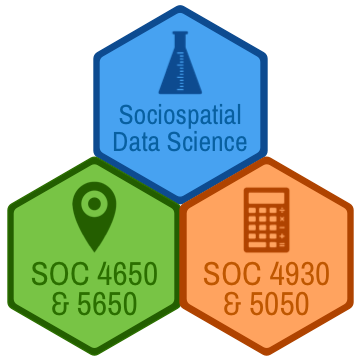
\includegraphics[width=0.4\linewidth]{images/SSDSBookBanner} \end{center}

This text is a companion text for both of my research methods courses at
\href{https://slu.edu}{Saint Louis University}:

\begin{itemize}
\tightlist
\item
  \href{https://slu-soc5650.github.io}{SOC 4650/5650 - Introduction to
  Geographic Information Science}
\item
  \href{https://slu-soc5050.github.io}{SOC 4930/5050 - Quantitative
  Analysis: Applied Inferential Statistics}
\end{itemize}

The goal of the text is to create a reference for the intangible, subtle
or disparate skills and ideas that contribute to being a successful
\emph{computational} social scientist. In writing this text, I draw
inspiration from the work of Donald Knuth.\footnote{\href{https://en.wikipedia.org/wiki/Donald_Knuth}{Donald
  Knuth} is the developer of
  \href{https://en.wikipedia.org/wiki/TeX}{TeX}, a computer typesetting
  system that is widely used today for scientific publishing in the form
  of \href{https://en.wikipedia.org/wiki/LaTeX}{LaTeX}. He also
  established the concept of
  \href{https://en.wikipedia.org/wiki/Literate_programming}{literate
  programming}, which forms the basis of some of the practices we follow
  with \texttt{R}.} Knuth has discussed his experiences in designing new
software languages, nothing that the developer of a new language

\begin{quote}
\ldots{}must not only be the implementer and the first large-scale user;
the designer should also write the first user manual\ldots{} If I had
not participated fully in all these activities, literally hundreds of
improvements would never have been made, because I would never have
thought of them or perceived why they were important\ldots{}
\end{quote}

While there is nothing particularly new about what I am writing here,
and I am certainly not developing a new language for computing, the goal
of this text remains similar to Knuth's experience. By distilling some
of key elements for making a successful transition to being a
\emph{professional developer} of knowledge rather than a \emph{casual
consumer}, I hope to both improve the course experience itself and also
create an environment that fosters a successful learning experience for
you.

In both classes, the course names are deceptive. We are not only
concerned with statistical work or mapping. Rather, we are more
fundamentally concerned with research methods. In particular, we are
concerned with \emph{high quality} research methods and the
\emph{process} of conducting research. We therefore focus on a
combination of mental habits and technical practices that make you a
successful researcher. Some of the skills and techniques that we will
discuss this semester are not taught as often in graduate programs, let
along undergraduate programs. Instead, they are often the products of
``learning the hard way''. These ``habits of mind and habits of method''
are broadly applicable across methodologies and disciplines.

\section*{License}\label{license}
\addcontentsline{toc}{section}{License}

Copyright © 2016-2017 \href{https://chris-prener.github.io}{Christopher
G. Prener}

This work is licensed under a Creative Commons Attribution 4.0
International License.

\chapter{Introduction}\label{intro}

The first part of this text is designed to help get you oriented to
coursework in computational social science. Both
\href{https://slu-soc5650.github.io}{Introduction to Geographic
Information Science (SOC 4650/5650)} and
\href{https://slu-soc5050.github.io}{Quantitative Analysis: Applied
Inferential Statistics (SOC 4930/5050)} are focused on building
students' capacities to address social science research questions using
tools that have been the traditional domain of computer and information
scientists. The growth and application of these tools in a variety of
disciplines both inside and outside of the social sciences has come to
be known as data science. Both courses are taught from this perspective,
so that while we focus on social science data, the tools and techniques
are broadly applicable across disciplines.

\section{What is data science?}\label{what-is-data-science}

Given data science's new emergence, its definition remains both
contested and often unclear. For me, there are four key aspects to focus
on when considering what constitutes data science:

\begin{enumerate}
\def\labelenumi{\arabic{enumi}.}
\tightlist
\item
  Statistics
\item
  Programming
\item
  Visualization and Communication
\item
  Substantive Knowledge
\end{enumerate}

I think of this as a ``full stack'' approach to computational research.
You want to be well versed not only the techniques for generating and
analyzing data, but also substantively in the academic literature about
your area of interest as well as ways to communicate your findings with
other researchers and the wider public.

\subsection{Statistics}\label{statistics}

Statistics covers the mathematical techniques that we use to draw
inference from our data. It is the main subject of one my courses,
\href{https://slu-soc5050.github.io}{Quantitative Analysis}. In
\href{https://slu-soc5650.github.io}{Introduction to GIS}, we do not
explicitly cover much in the way of inferential statistics. However, the
course is desinged to prepare you for a next level, Intermediate GIS
course that covers spatial statistics.

\subsection{Programming}\label{programming}

Computer programming is an essential part of data science broadly and
computational social science more specifically. Using a programming
language means that our work can be easily reproduced. This emphasis on
\textbf{reproducibility} is a response to a growing fear in many
disciplines that results are replicable from study to study, which
raises questions about the validity of much of the research work that we
do. Our goal in both courses is to produce research that is as
reproducible as possible.

This book introduces two programming languages -
\href{https://en.wikipedia.org/wiki/R_(programming_language)}{\texttt{R}}
and
\href{https://en.wikipedia.org/wiki/Python_(programming_language)}{Python}.
In \href{https://slu-soc5050.github.io}{Quantitative Analysis}, we will
be focused exclusively on learning \texttt{R} and using it to produce
statistical analyses. In
\href{https://slu-soc5650.github.io}{Introduction to GIS}, we will spend
a lot of time in \texttt{R}, but we will also use some Python to help
pass data from \texttt{R} to ArcGIS, the mapping application we will
use. I will also provide some additional Python lessons to folks who are
interested, but these will not be required for the course.

\subsection{Visualization \&
Communication}\label{visualization-communication}

Visualization is a fundamental aspect of data science work. It is how we
make our results easily digestible and accessible to a wider audience,
many of whom may not be able to interpret statistical output but can
learn from a well-designed scatter plot. In
\href{https://slu-soc5050.github.io}{Quantitative Analysis}, we will
focus on building plots to communicate information about statistical
distributions and the relationships between our variables. In
\href{https://slu-soc5650.github.io}{Introduction to GIS}, we will use
the same fundamental skills to build simple maps in \texttt{R}. We will
extend our emphasis on visualization to ArcGIS, where we will focus on
producing cartographically rich depictions of our data.

Separetely, we will discuss the presentation of statistical data in
tables using \href{https://en.wikipedia.org/wiki/LaTeX}{LaTex} in
\href{https://slu-soc5050.github.io}{Quantitative Analysis} as well as
the producing to conference-style presentations to communicate research
findings. In \href{https://slu-soc5650.github.io}{Introduction to GIS},
we will focus on producing conference-style posters instead. These are
different mediums, but they rely on the same design fundamentals that
are covered in this text.

\subsection{Substantive Knowledge}\label{substantive-knowledge}

Substantive knowledge covers two tangentially related topics: the
ability to work well in groups and the ability to digest and integrate
an academic literature into your own research. Each of these topics
receive some focus in both
\href{https://slu-soc5050.github.io}{Quantitative Analysis} and
\href{https://slu-soc5650.github.io}{Introduction to GIS}. Each class
has some group work associated with the completion with weekly lab
assignments. \href{https://slu-soc5650.github.io}{Introduction to GIS}
also has a group work component associated with the final project. In
each class, students' final projects are focused on a specific content
area that requires at least some background research and knowledge.
Synthesizing this knowledge and integrating it into your final projects
is a key piece of addressing this facet of data science.

\part{First Steps}\label{part-first-steps}

\chapter{Getting Started}\label{gettingStarted}

Before you begin the semester, there are a number of things that I
recommend that you do to help set yourself up for success. Before you do
\emph{anything} else, you should read through the
\href{https://cdn.rawgit.com/slu-soc5050/Core-Documents/bdcce556/syllabus.pdf}{\textbf{Syllabus}}
and the
\href{https://cdn.rawgit.com/slu-soc5050/Core-Documents/bdcce556/reading-list.pdf}{\textbf{Reading
List}}. Make sure you have a good sense of what is \emph{required} for
the course. If you have questions, bring them to the first day of class!

\section{Account Signups}\label{account-signups}

\subsection{Get Started with Slack}\label{get-started-with-slack}

We'll be using the messaging platform \href{https://slack.com}{Slack} as
a space for ``virtual office hours''. Slack is a messaging system used
by teams of all kinds. If you can text, you can use Slack. You will need
to sign-up for the SOC 5050 Slack organization
\href{https://join.slack.com/t/slu-soc5050/signup}{here}. You will need
to complete the signup process even if you use Slack for other purposes.
Consider installing either the desktop or the mobile apps for Slack to
keep in touch and receive push alerts!

\subsection{Get Started with GitHub}\label{get-started-with-github}

The website that is hosting this wiki is called
\href{https://github.com/}{GitHub}. GitHub is used by programmers, data
scientists, and researchers for hosting computer code, data, and project
materials. We will be using GitHub extensively this semester. You will
need a free account, which you can sign up for one from GitHub's
\href{https://github.com/}{homepage}. If you already have a GitHub
account, you do not need a new one. \emph{Once you have a GitHub user
name, send Chris a Direct Message via Slack with it so that you can be
added to the SOC 5050 organization.}

\subsection{Get Started with LaTeX}\label{get-started-with-latex}

We'll be doing a little bit of writing using LaTeX, which is a markup
language that makes technical writing easier. We'll be using
\href{https://www.sharelatex.com}{ShareLaTeX} this semester for this
purpose. ShareLaTeX is a bit like Google Docs, but for LaTeX. It is a
``freemium'' service - please don't pay for any additional features -
you won't need them! You can sign-up for ShareLaTeX on their
\href{https://www.sharelatex.com}{website}.

\section{Get Started with Software}\label{get-started-with-software}

If you will be using your own computer in class, you'll want to install
a number of applications. If you aren't using your own computer, you can
skip this section! All of these applications are available in our
classroom, and - lucky you - you get 24-hour access to Morrissey Hall
for the semester.

\subsection{Computer Prep}\label{computer-prep}

Before you install your software, you should do the following:

\begin{enumerate}
\def\labelenumi{\arabic{enumi}.}
\item
  Make sure your operating system is up-to-date. If you are able, I
  would also recommend upgrading your computer to the most recent
  release of its operating system that the computer can run.
\item
  We'll be sharing computer files throughout the semester, so you should
  ensure that you have functioning anti-virus software and that it is
  up-to-date. You can get anti-virus software for free from SLU. Go to
  \texttt{ITS\ Software\ Downloads} under \texttt{Tools} on
  \href{https://myslu.slu.edu/tools}{mySLU}.
\item
  You'll also need to download files, so you'll need to make sure you
  have some free space on your hard drive. If you have less than 10GB of
  free space, you should de-clutter!
\item
  Make sure you know how to access your computer's file management
  system.
\end{enumerate}

\begin{itemize}
\tightlist
\item
  On macOS, this means being comfortable with Finder.app.
\item
  On Windows, this means being comfortable with Windows Explorer.
\end{itemize}

\subsection{Software Installation}\label{software-installation}

Now that your computer is up-to-date

\begin{enumerate}
\def\labelenumi{\arabic{enumi}.}
\item
  The computing language \texttt{R} needs to be downloaded and
  installed. You can download it from the
  \href{https://cran.cnr.berkeley.edu}{University of
  California-Berkeley}. Choose ``Download R for (Mac) OS X'' or
  ``Download R for Windows''.
\item
  RStudio is a graphical user interface for \texttt{R} that will make
  learning the language and using it much, much easier. You should
  download the \emph{free} version of RStudio from
  \href{https://www.rstudio.com/products/rstudio/download/\#download}{their
  website}. Choose the installer for your platform, and ping me on Slack
  if you have any questions.
\item
  GitHub Desktop is a client for interacting with GitHub that makes
  downloading and uploading files a breeze. You can download it from the
  developer's \href{http://desktop.github.com}{website}.
\item
  Atom is a text editor that is produced by the same folks who operate
  GitHub. Download Atom from the developer's
  \href{http://atom.io}{website}.
\end{enumerate}

\section{Get Access to Books and
Readings}\label{get-access-to-books-and-readings}

\subsection{Books}\label{books}

There are three books required for this course. Each book has been
selected to correspond with one or more of the course objectives. The
books are:

\begin{enumerate}
\def\labelenumi{\arabic{enumi}.}
\item
  Freedman, David, Robert Pisani, and Roger Purves. 2007.
  \emph{Statistics}. 4th edition. New York, NY: W.W. Norton and Company.
\item
  Wheelan, Charles. 2014. \emph{Naked Statistics: Stripping the Dread
  from the Data}. New York, NY: W.W. Norton and Company.
\item
  Wickham, Hadley and Garrett Grolemund. 2016. \emph{R for data
  science}. Sebastopol, CA: O'Reilly.
  \href{http://r4ds.had.co.nz}{Webbook Available}.
\end{enumerate}

All of the books are available in the bookstore. They can also be
ordered online. If you would rather use ebooks, those are acceptable for
this course as well.

\subsection{Check Out the Readings for Week
01}\label{check-out-the-readings-for-week-01}

All but one of the Week 01 readings are available on our course's
\href{http://eres.slu.edu/eres/coursepass.aspx?cid=4487}{electronic
reserves site}, and the password is posted in Slack on the
\texttt{\#helpdesk-coursework} channel. The initial section of Wickham
and Grolemund can be found via the
\href{http://r4ds.had.co.nz}{webbook}.

\section{Administrative Tasks}\label{administrative-tasks}

There are two forms that all students must fill out by Tuesday,
September 5th:

\begin{enumerate}
\def\labelenumi{\arabic{enumi}.}
\item
  the \href{https://goo.gl/forms/HddqLWd00qz6Qs903}{Student Information
  Sheet}, which gives me some info about you and gives you the chance to
  let me know about any initial concerns you might have.
\item
  the un-graded \href{https://goo.gl/forms/EgVGaUWu8mys2yBr2}{Diagnostic
  Assessment}, which is designed to get a sense of where each student's
  math skills are currently. Please don't consult outside materials as
  you do this - if you are not sure how to answer, make the most
  educated guess you can and move on. If you look answers up it defeats
  the purpose of this exercise!
\end{enumerate}

\bibliography{packages.bib,book.bib}


\end{document}
